\section{Sequence Imminence}{\label{sec:sequences}}
\begin{topics}
\verb!array! traversal, manipulation and previous sections. Some problems can be solved without arrays too.
\end{topics}
% \begin{note}
% 	This is the last problem set where we use Simplecpp. We will move onto C++ from the next problem set.
% \end{note}
\subsection{Josephus Problem}
Suppose there are $n$ terrorists around a circle facing towards the centre. They are numbered $1$ to $n$ along clockwise direction. Initially, terrorist 1 has the sword. Now, the terrorist with sword kills the $k$\textsuperscript{th} nearest alive terrorist to its left and passes the sword to $(k+1)$\textsuperscript{st} nearest alive terrorist to its left. The process repeats. Basically, every $k$\textsuperscript{th} terrorist is killed until only one survives. Then the last terrorist is killed.
\begin{figure}[H]
    \centering
    
\includegraphics[width = 0.15\linewidth]{Josephus.pdf}
    \caption{Example arrangement of 10 terrorists}
    \label{fig:jp}
\end{figure}
\vspace{-1.5em}
For example, in the above arrangement,\\
when $k=1,$ 1 kills 2, 3 kills 4, 5 kills 6, 7 kills 8, 9 kills 10, 1 kills 3, 5 kills 7, 9 kills 1 and 5 kills 9. So, 5 survives;\\% and is killed last;\\
when $k=2,$ 1 kills 3, 4 kills 6, 7 kills 9, 10 kills 2, 4 kills 7, 8 kills 1, 4 kills 8, 10 kills 5 and 4 kills 10. So, 4 survives.\\% and is killed last.
\textbf{Problem Statement:}\\
For a given $n, k$ pair, and starting position $1$, print the terrorists in the sequence they are killed.
\begin{testcases}
	{$t$ \hfill(number of test cases, an integer)\\
	$n_1\ k_1\ \quad n_2\ k_2\ \quad \ldots\quad n_t\ k_t$ \hfill($t$ space seperated pairs (number of terrorists $n$ and $k$) for each testcase)}
	{Terrorists in the sequence they are killed \hfill(each test case on a newline)}
	{$1 \leq k_i \leq n_i \leq 100$}
	{9\\1 1\quad2 1\quad4 1\quad4 2\quad8 1\quad8 3\quad10 2\quad16 7\quad50 25}
	{1\\2 1\\2 4 3 1\\3 2 4 1\\2 4 6 8 3 7 5 1\\4 8 5 2 1 3 7 6\\3 6 9 2 7 1 8 5 10 4\\8 16 9 2 12 6 3 15 14 1 5 11 10 4 13 7\\26 2 29 6 34 12 41 20 50 32 14 46 30 15 49 37 23 11 3 43 36 28 24 21 19 22 27 35 42 1 10 33 4 25 7 44 38 31 40 5 18 16 39 9 17 45 48 13 8 47}
	{https://github.com/paramrathour/CS-101/tree/main/Starter Codes/Josephus Problem.cpp}
\end{testcases}
\begin{note}
	Verify your program on even more testcases from \href{https://cses.fi/problemset/task/2163/}{here}.
\end{note}
\begin{funvideo}
	\href{https://youtu.be/uCsD3ZGzMgE}{The Josephus Problem -- Numberphile}
\end{funvideo}
\subsection{Van Eck's Sequence}
The Van Eck's Sequence is defined as follows:
\begin{itemize}
	\item $a_0 = 0$ then for $n>0$,\\
	\item $a_{n+1} = \begin{cases}
		n-m & \text{where $m$ the maximal index $<n$ exists, such that $a_{m}=a_{n}$}\\
		0 & \text{if such $m<n$ doesn't exist, then we take $m=n\ \rightarrow\ a_{n+1}=0$.}
	\end{cases}$
\end{itemize}
\textbf{Problem Statement:}\\
Generate the first $n+1$ elements $a_0,a_1,\ldots,a_n$ of the Van Eck's Sequence.
\begin{testcasesMore}
	{$n$ \hfill(a single integer)}
	{$a_0\ a_1\ \ldots\ a_n$\hfill(space seperated integers)}
	{$1 \leq n \leq 100000$}
	{500}
	{0 0 1 0 2 0 2 2 1 6 0 5 0 2 6 5 4 0 5 3 0 3 2 9 0 4 9 3 6 14 0 6 3 5 15 0 5 3 5 2 17 0 6 11 0 3 8 0 3 3 1 42 0 5 15 20 0 4 32 0 3 11 18 0 4 7 0 3 7 3 2 31 0 6 31 3 6 3 2 8 33 0 9 56 0 3 8 7 19 0 5 37 0 3 8 8 1 46 0 6 23 0 3 9 21 0 4 42 56 25 0 5 21 8 18 52 0 6 18 4 13 0 5 11 62 0 4 7 40 0 4 4 1 36 0 5 13 16 0 4 8 27 0 4 4 1 13 10 0 6 32 92 0 4 9 51 0 4 4 1 14 131 0 6 14 4 7 39 0 6 6 1 12 0 5 39 8 36 44 0 6 10 34 0 4 19 97 0 4 4 1 19 6 12 21 82 0 9 43 0 3 98 0 3 3 1 15 152 0 6 17 170 0 4 24 0 3 12 24 4 6 11 98 21 29 0 10 45 0 3 13 84 0 4 14 70 0 4 4 1 34 58 0 6 23 144 0 4 9 51 94 0 5 78 0 3 26 0 3 3 1 21 38 0 6 21 4 19 76 0 6 6 1 12 56 166 0 7 111 0 3 21 16 145 0 5 33 206 0 4 23 46 194 0 5 9 47 0 4 9 4 2 223 0 6 33 19 39 132 0 6 6 1 40 185 0 6 5 23 28 0 5 4 22 0 4 3 46 36 151 0 6 15 126 0 4 10 110 0 4 4 1 29 118 0 6 14 112 0 4 9 51 102 0 5 33 50 0 4 9 9 1 20 307 0 7 88 0 3 42 262 0 4 14 27 233 0 5 23 60 0 4 9 22 60 5 8 210 0 8 3 22 8 3 3 1 34 156 0 10 63 0 3 8 11 183 0 5 22 17 199 0 5 5 1 19 109 0 6 73 0 3 19 7 58 183 20 64 0 8 26 174 0 4 52 319 0 4 4 1 25 331 0 6 25 4 7 23 69 0 7 4 6 9 71 0 6 4 6 2 158 0 6 4 6 2 6 2 2 1 30 0 10 73 54 0 4 13 247 0 4 4 1 13 6 18 367 0 8 59 0 3 70 257 0 4 14 123 0 4 4}
	{https://github.com/paramrathour/CS-101/tree/main/Test Cases/Van Eck's Sequence/Input.txt}
	{https://github.com/paramrathour/CS-101/tree/main/Test Cases/Van Eck's Sequence/Output.txt}
	{https://github.com/paramrathour/CS-101/tree/main/Starter Codes/Van Eck's Sequence.cpp}
\end{testcasesMore}
\begin{funvideo}
	\href{https://youtu.be/etMJxB-igrc}{Don't Know (the Van Eck Sequence) -- Numberphile}
\end{funvideo}
\subsection{Look-And-Say Sequence}
As the name suggests, the look-and-say sequence is generated by the \emph{reading} of the digits of the previous sequence.\\% in a \emph{look-and-say manner}.\\
For example, starting with the sequence \textbf{1}.
\begin{itemize}
\item \textbf{1} is read off as ``one 1'' or \textbf{11}.
\item \textbf{11} is read off as ``two 1s'' or \textbf{21}.
\item \textbf{21} is read off as ``one 2, one 1'' or \textbf{1211}.
\item \textbf{1211} is read off as ``one 1, one 2, two 1s'' or \textbf{111221}.
\item \textbf{111221} is read off as ``three 1s, two 2s, one 1'' or \textbf{312211} and so on.
\end{itemize}
\textbf{Problem Statement:}\\
Generate the first $n$ iterations of the look-and-say sequence.
\begin{testcasesMore}
	{$n$ \hfill(a single integer)}
	{First $n$ iterations of the look-and-say sequence\hfill(each iteration on a newline)}
	{$1 \leq n \leq 40$}
	{15}
	{1\\[0.5em]11\\[0.5em]21\\[0.5em]1211\\[0.5em]111221\\[0.5em]312211\\[0.5em]13112221\\[0.5em]1113213211\\[0.5em]31131211131221\\[0.5em]13211311123113112211\\[0.5em]11131221133112132113212221\\[0.5em]3113112221232112111312211312113211\\[0.5em]1321132132111213122112311311222113111221131221\\[0.5em]11131221131211131231121113112221121321132132211331222113112211\\[0.5em]311311222113111231131112132112311321322112111312211312111322212311322113212221}
	{https://github.com/paramrathour/CS-101/tree/main/Test Cases/Look-And-Say Sequence/Input.txt}
	{https://github.com/paramrathour/CS-101/tree/main/Test Cases/Look-And-Say Sequence/Output.txt}
	{https://github.com/paramrathour/CS-101/tree/main/Starter Codes/Look-And-Say Sequence.cpp}
\end{testcasesMore}
\begin{funvideo}
	\href{https://youtu.be/ea7lJkEhytA}{Look-and-Say Numbers (feat John Conway) -- Numberphile}
\end{funvideo}
\KOMAoptions{paper=A3}
\recalctypearea
\subsection{Thue-Morse Sequence}{\label{pp:thuemorsesequence}}
Thue-Morse Sequence aka Fair Share Sequence is an infinite binary sequence obtained by starting with 0 and successively appending the Boolean complement of the sequence obtained thus far (called prefixes of the sequence).\\
For example, starting with the sequence \textbf{0},
\begin{itemize}
	\item Append complement of \textbf{0}, we get 0\textbf{1}
	\item Append complement of \textbf{01}, we get 01\textbf{10}
	\item Append complement of \textbf{0110}, we get 0110\textbf{1001} and so on.
\end{itemize}
Also, by using Thue-Morse sequence elements in the turtle simulator, we get a mysterious curve\footnote{called Koch curve, it is a fractal curve that has infinite length but contained in a finite area. Can you see why?} by following the below rule.
\begin{itemize}
	\item If an element is 0, then the turtle rotates \verb!right! by 180\textdegree.
	\item If an element is 1, then the turtle moves \verb!forward! by one unit and then rotates \verb!right! by 60\textdegree.
\end{itemize}
Can you figure out the pattern of this curve?

\textbf{Problem Statement:}\\
Generate the first $n$ elements of the Thue-Morse sequence and draw the corresponding curve using \verb!turtleSim!.\\
Scale the curve in such a way that it roughly takes same width and height for all $n$.
% \begin{testcasesMore}
% 	{$t$ \hfill(number of test cases, an integer)\\
% 	$n_1\ n_2\ \ldots n_t$ \hfill($t$ space seperated integers for each testcase)}
% 	{First $n_i$ elements of the Thue-Morse sequence and the curve.\hfill(each testcase on a newline)}
% 	{$1 \leq n_i \leq 100000$ ($n_i$ need not be a power of 2)}
% 	{4\\2 32 111 128}
% 	{01\\01101001100101101001011001101001\\011010011001011010010110011010011001011001101001011010011001011010010110011010010110100110010110011010011001011\\01101001100101101001011001101001100101100110100101101001100101101001011001101001011010011001011001101001100101101001011001101001}
% 	{https://github.com/paramrathour/CS-101/tree/main/Test Cases/Thue-Morse Sequence/Input.txt}
% 	{https://github.com/paramrathour/CS-101/tree/main/Test Cases/Thue-Morse Sequence/Output.txt}
% 	{https://github.com/paramrathour/CS-101/tree/main/Starter Codes/Thue-Morse Sequence.cpp}
% \end{testcasesMore}
\begin{testcasesMore}
	{$n$ \hfill(a single integer)}
	{First $n$ elements of the Thue-Morse sequence and the curve.}
	{$1 \leq n \leq 100000$ ($n$ need not be a power of 2)}
	{111}
	{011010011001011010010110011010011001011001101001011010011001011010010110011010010110100110010110011010011001011}
	{https://github.com/paramrathour/CS-101/tree/main/Test Cases/Thue-Morse Sequence/Input.txt}
	{https://github.com/paramrathour/CS-101/tree/main/Test Cases/Thue-Morse Sequence/Output.txt}
	{https://github.com/paramrathour/CS-101/tree/main/Starter Codes/Thue-Morse Sequence.cpp}
\end{testcasesMore}
\textbf{The output Koch Curve convergents}
\begin{figure}[H]
	\centering
	\begin{subfigure}{0.3\linewidth}
		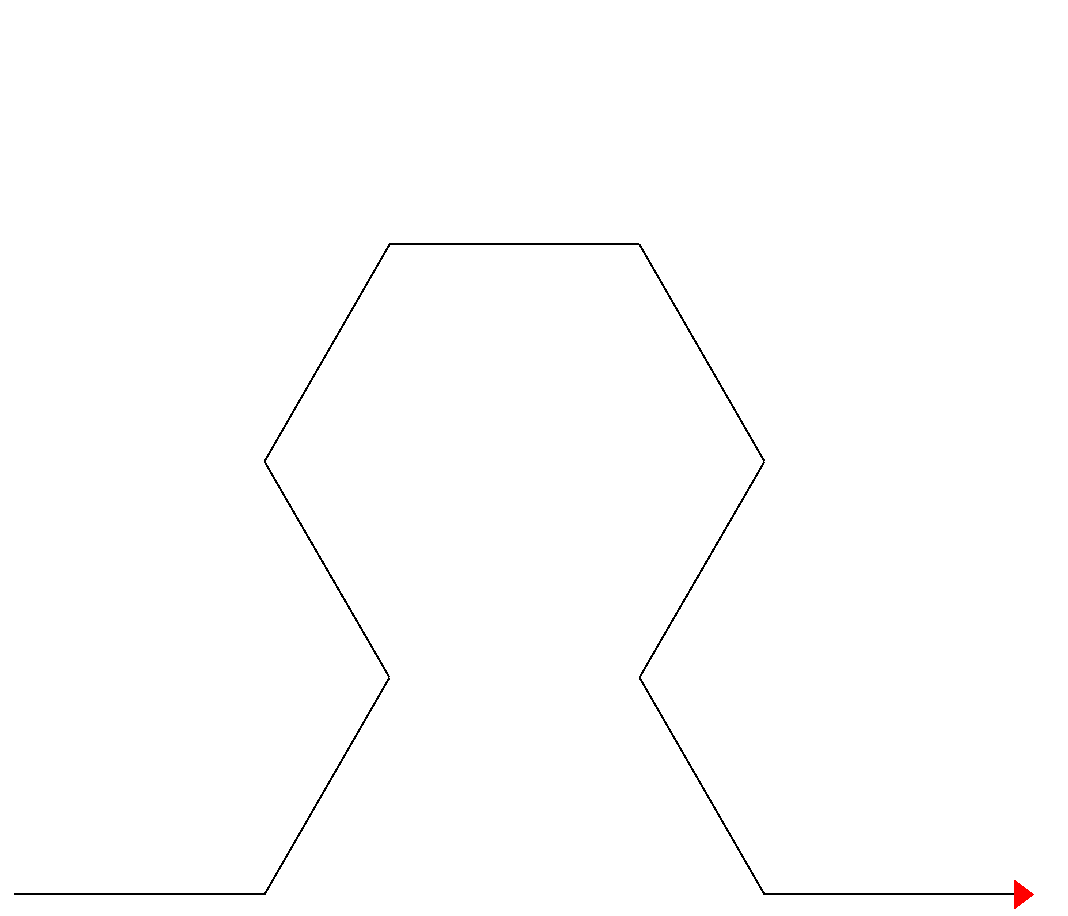
\includegraphics[width = \linewidth]{Thue-Morse Sequence/2.png}
		\caption{Iteration 0, $n=2$}
	\end{subfigure}
	\begin{subfigure}{0.3\linewidth}
		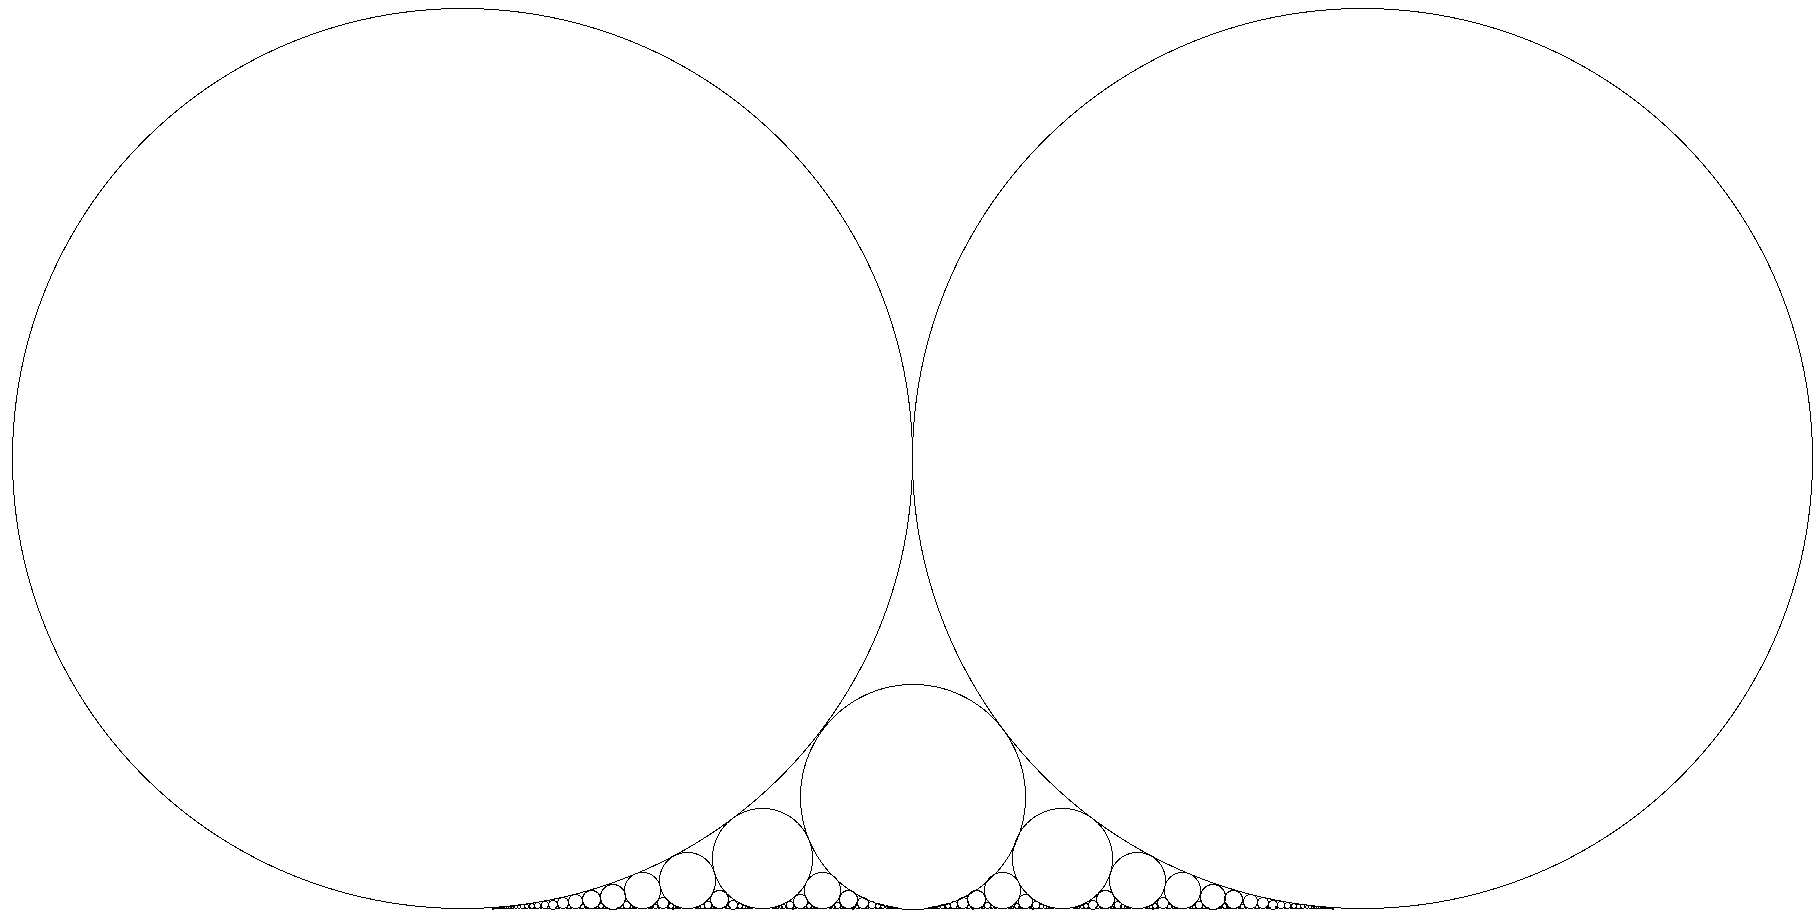
\includegraphics[width = \linewidth]{Thue-Morse Sequence/8.png}
		\caption{Iteration 1, $n=8$}
	\end{subfigure}
	\begin{subfigure}{0.3\linewidth}
		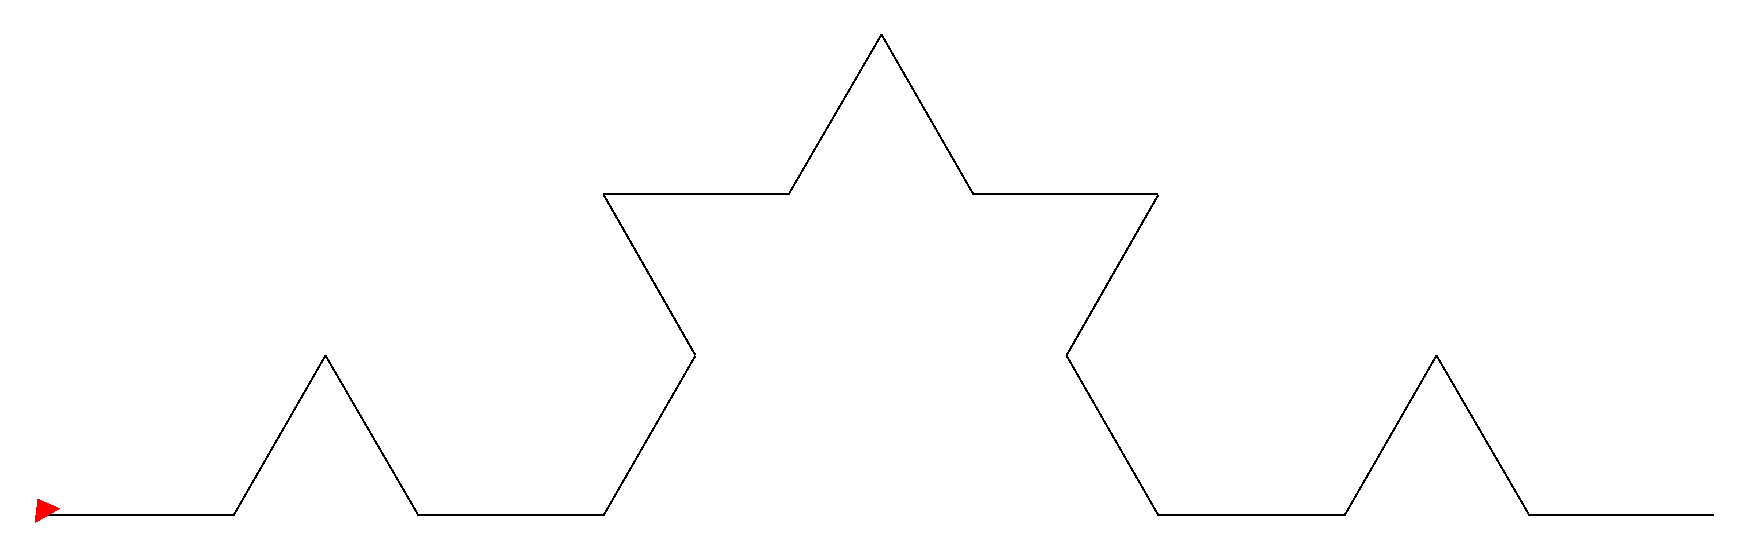
\includegraphics[width = \linewidth]{Thue-Morse Sequence/32.png}
		\caption{Iteration 2, $n=32$}
	\end{subfigure}
	\begin{subfigure}{0.3\linewidth}
		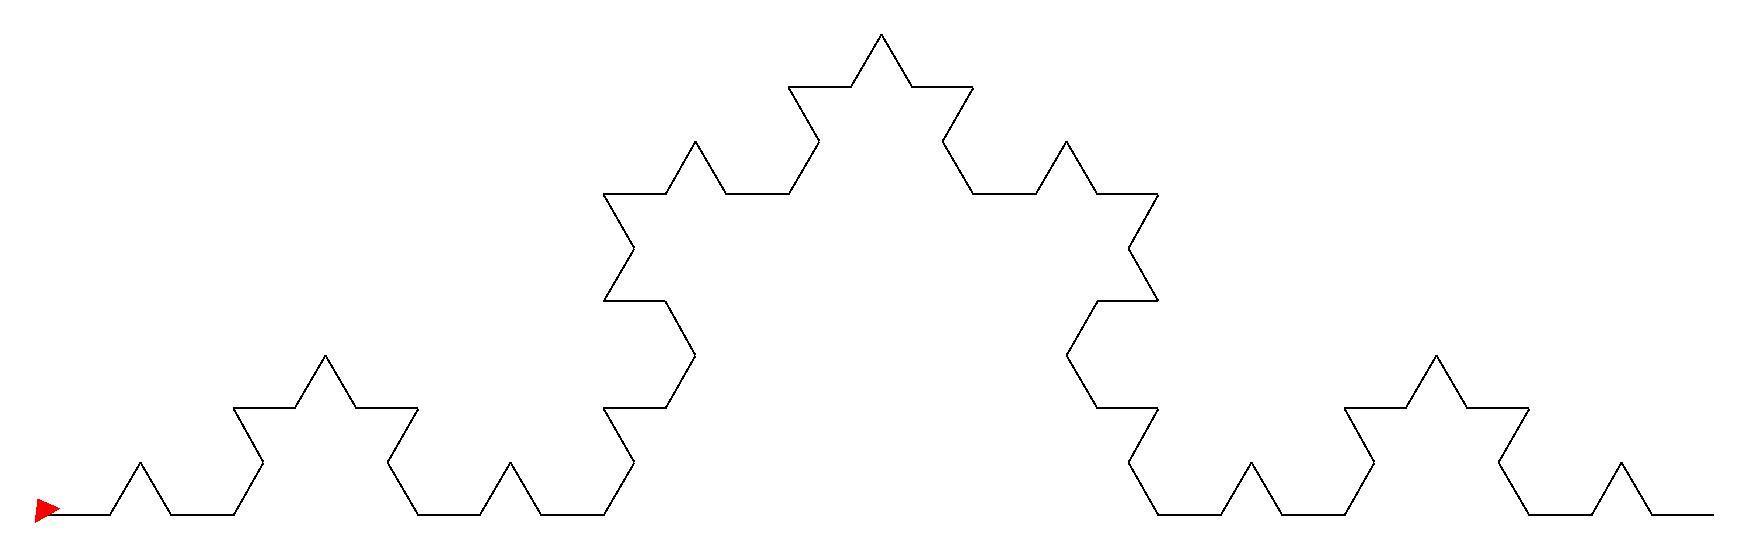
\includegraphics[width = \linewidth]{Thue-Morse Sequence/128.png}
		\caption{Iteration 3, $n=128$}
	\end{subfigure}
	\begin{subfigure}{0.3\linewidth}
		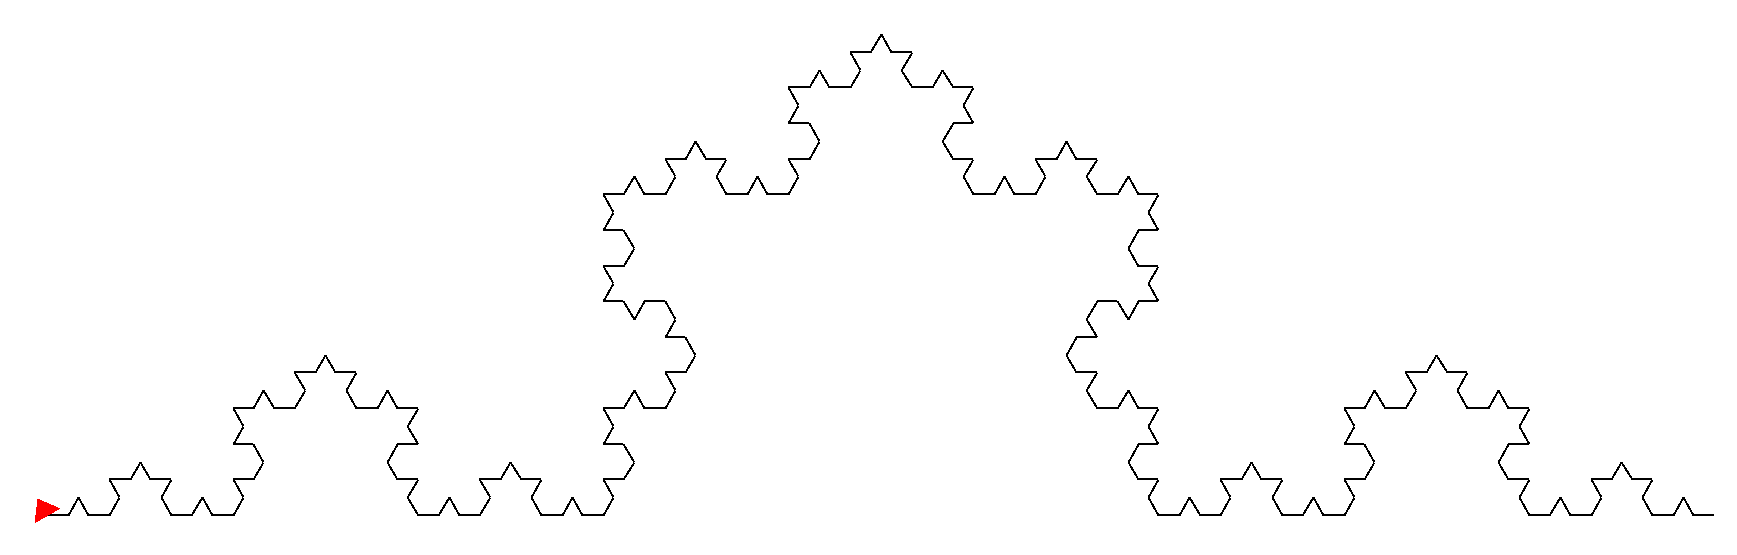
\includegraphics[width = \linewidth]{Thue-Morse Sequence/512.png}
		\caption{Iteration 4, $n=512$}
	\end{subfigure}
	\begin{subfigure}{0.3\linewidth}
		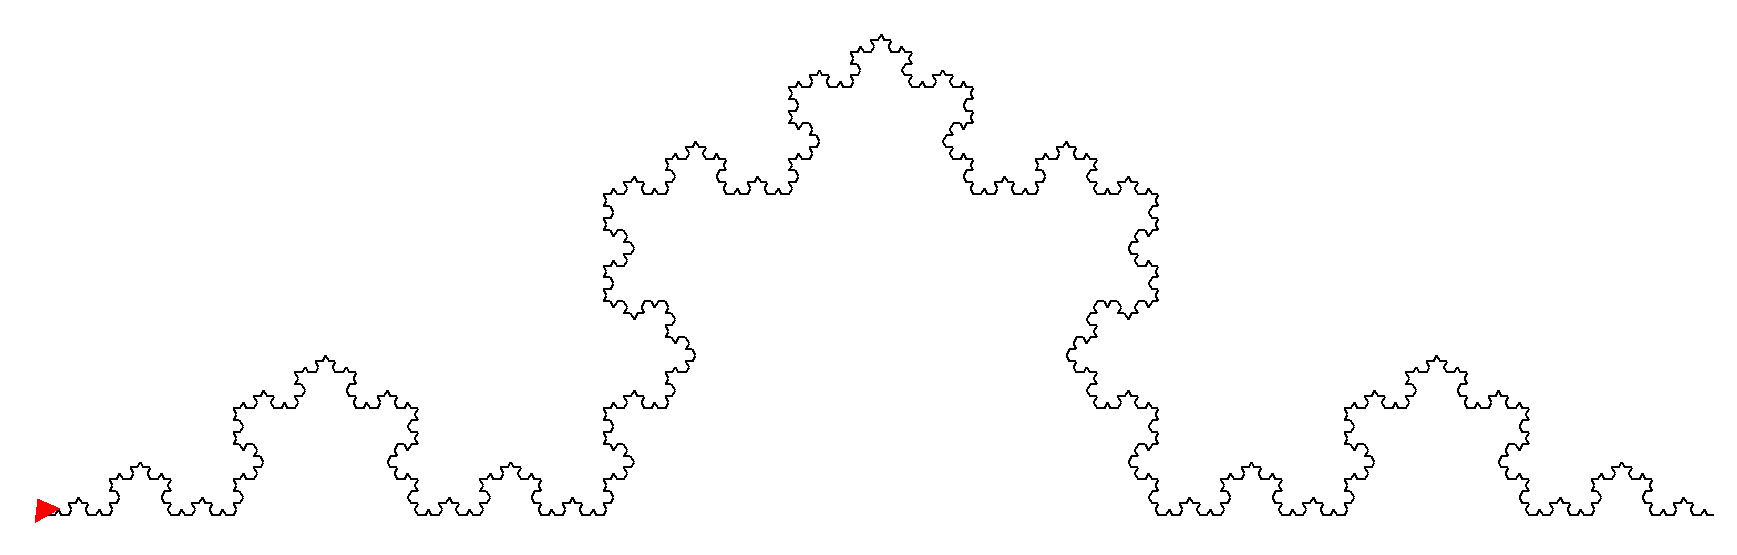
\includegraphics[width = \linewidth]{Thue-Morse Sequence/2048.png}
		\caption{Iteration 5, $n=2048$}
	\end{subfigure}
	\begin{subfigure}{0.3\linewidth}
		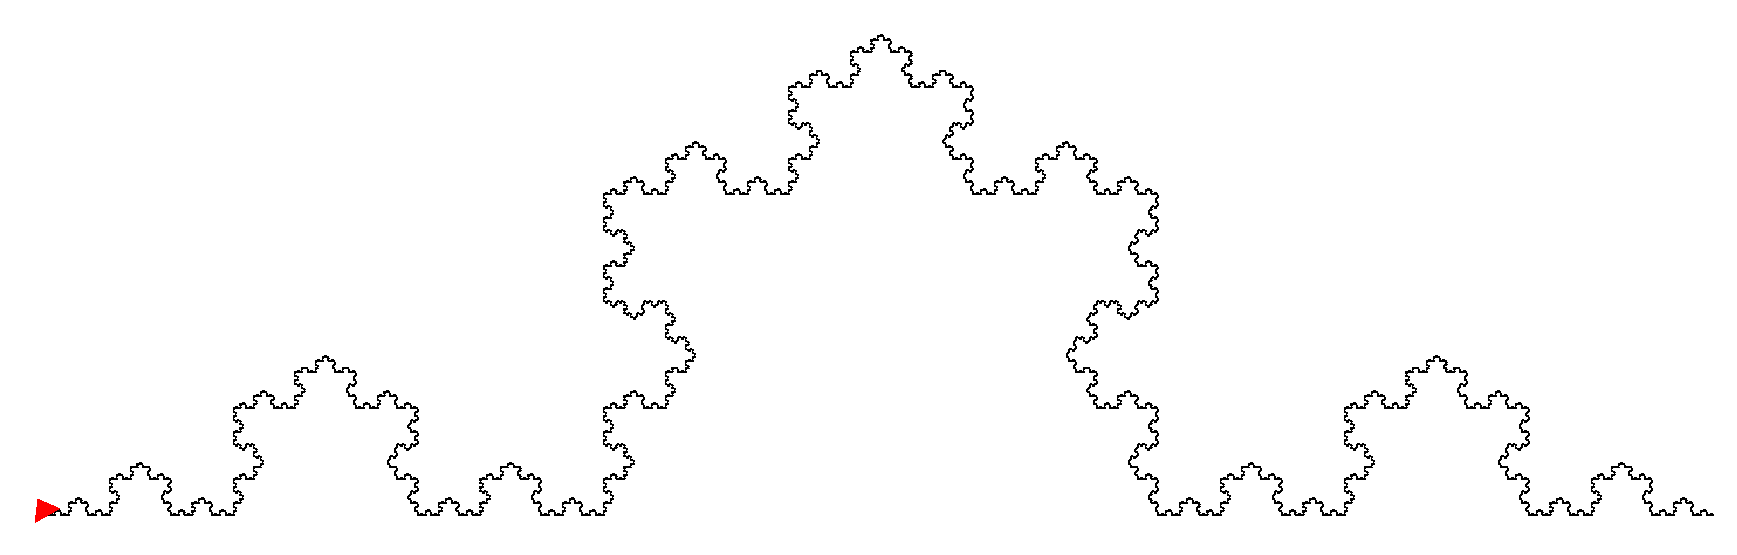
\includegraphics[width = \linewidth]{Thue-Morse Sequence/8192.png}
		\caption{Iteration 6, $n=8192$}
	\end{subfigure}
	\caption{Koch Curve Iterations and the outputs for odd powers of 2}
\end{figure}
\begin{figure}[H]
	\centering
	\begin{subfigure}{0.3\linewidth}
		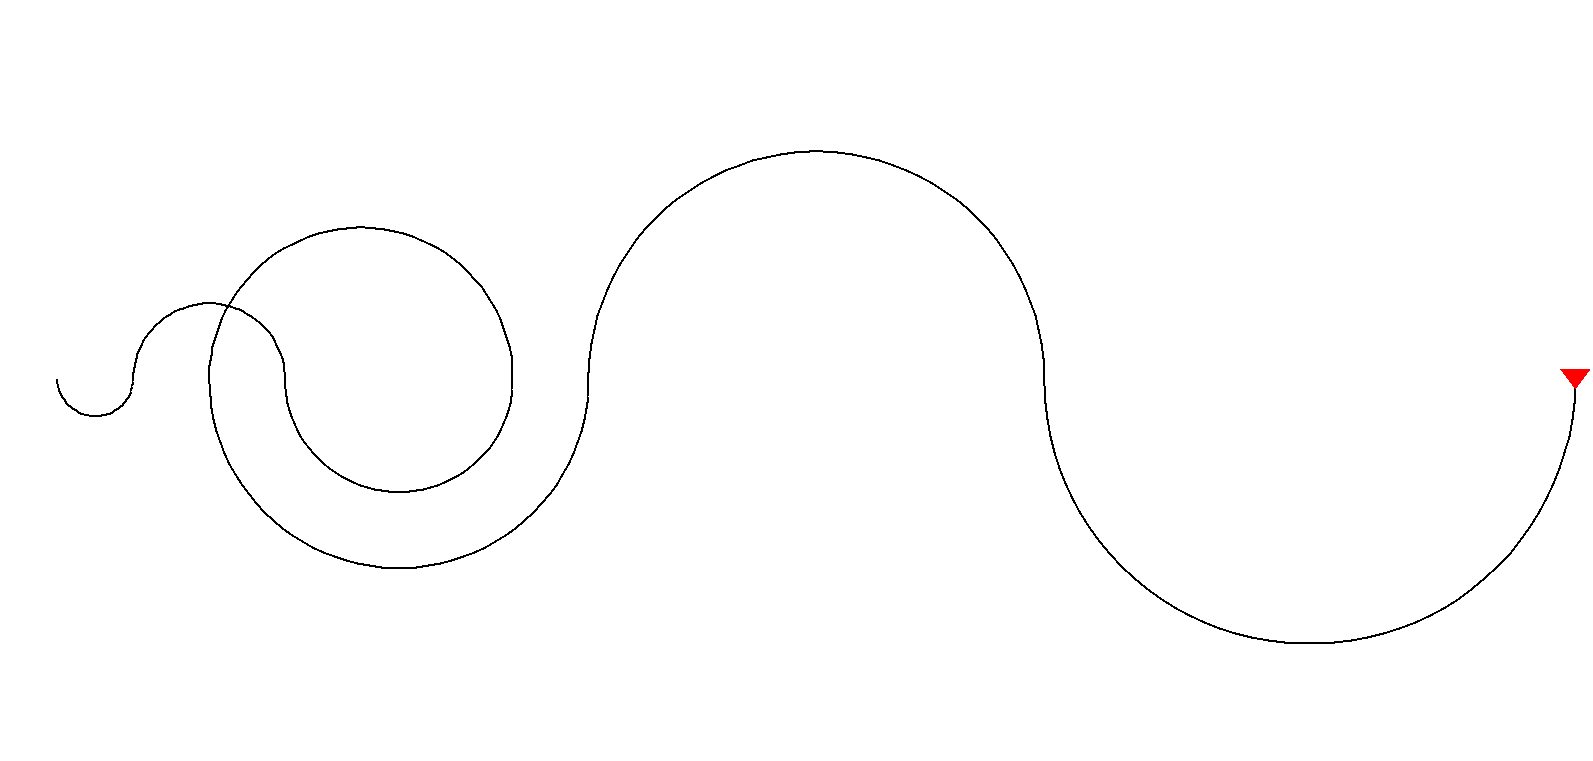
\includegraphics[width = \linewidth]{Thue-Morse Sequence/4.png}
		\caption{$n=4$}
	\end{subfigure}
	\begin{subfigure}{0.3\linewidth}
		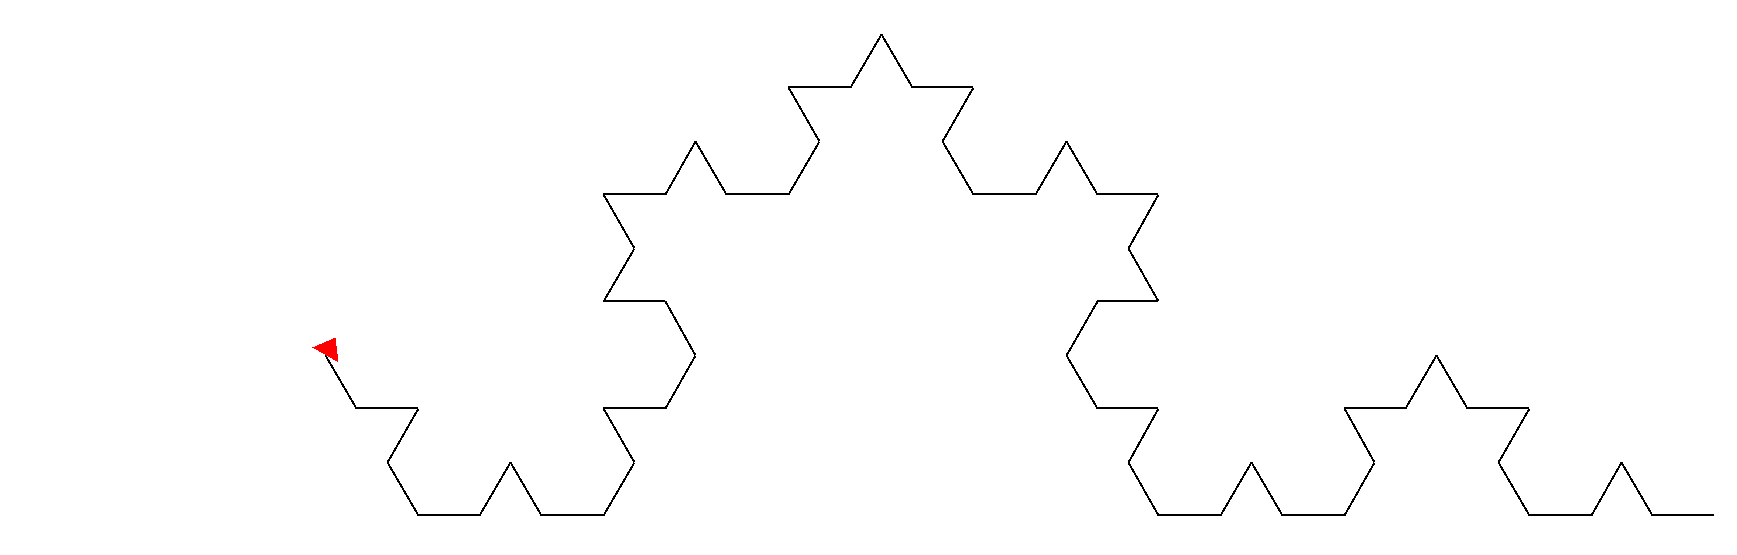
\includegraphics[width = \linewidth]{Thue-Morse Sequence/111.png}
		\caption{$n=111$}
	\end{subfigure}
	\begin{subfigure}{0.3\linewidth}
		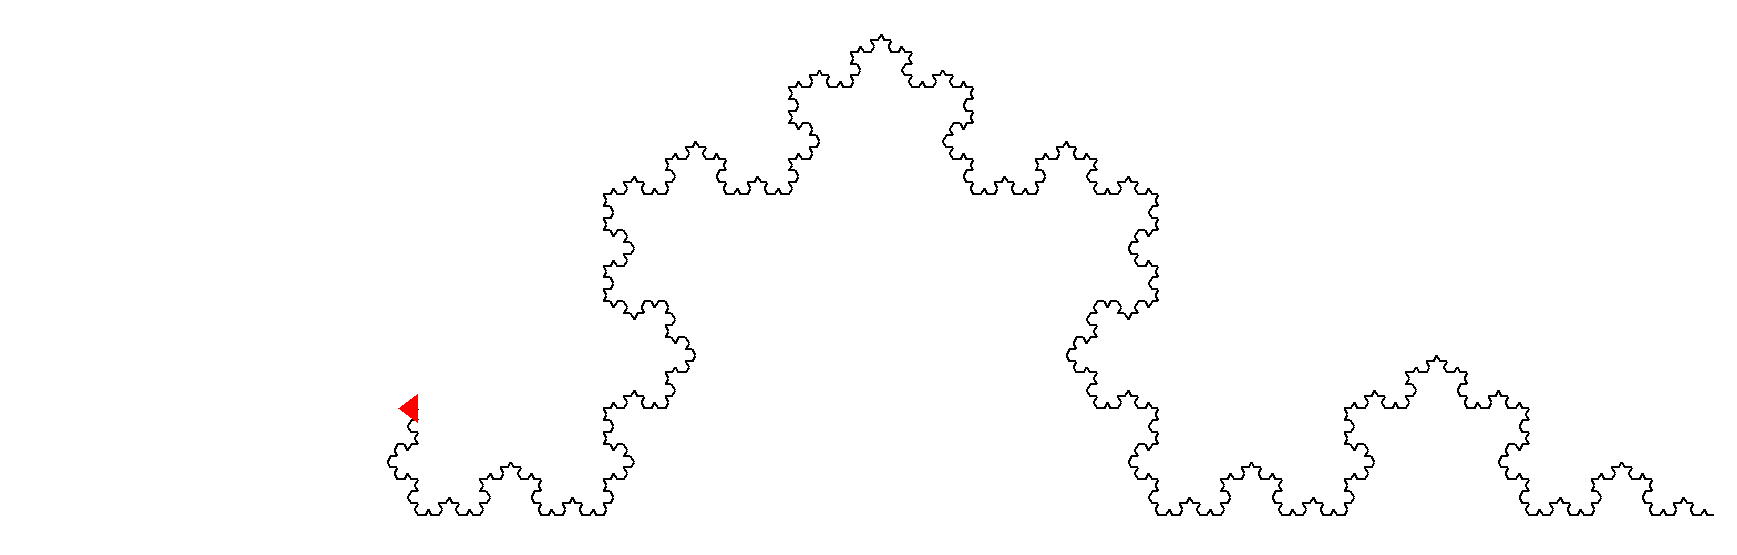
\includegraphics[width = \linewidth]{Thue-Morse Sequence/1729.png}
		\caption{$n=1729$}
	\end{subfigure}
	\caption{The outputs for numbers which are not a odd power of 2}
\end{figure}
\begin{funvideo}
	\href{https://youtu.be/prh72BLNjIk}{The Fairest Sharing Sequence Ever -- Stand-up Maths}\\
	\href{https://youtu.be/gB9n2gHsHN4}{Fractals are typically not self-similar -- 3Blue1Brown}
\end{funvideo}
\subsection{Recaman's Sequence}{\label{pp:recamanssequence}}
The Recaman's sequence is defined as below:
\begin{itemize}
	\item $r_0 = 0$
	\item $r_n = \begin{cases}
		r_{n-1} - n & \text{if } r_{n-1}-n>0 \text{ and } \forall i <n,\ r_i\neq r_{n-1}-n, \text{ i.e. $r_{n-1}-n$ is positive and has not yet occurred in the sequence}\\
		r_{n-1} + n & \text{otherwise}
	\end{cases}$
\end{itemize}
Also, by using Recaman's sequence elements in the turtle simulator, we can get beautiful curves as shown in \ref{fig:recamanssequence} by following the below rules:
\begin{figure}[H]
	\centering
	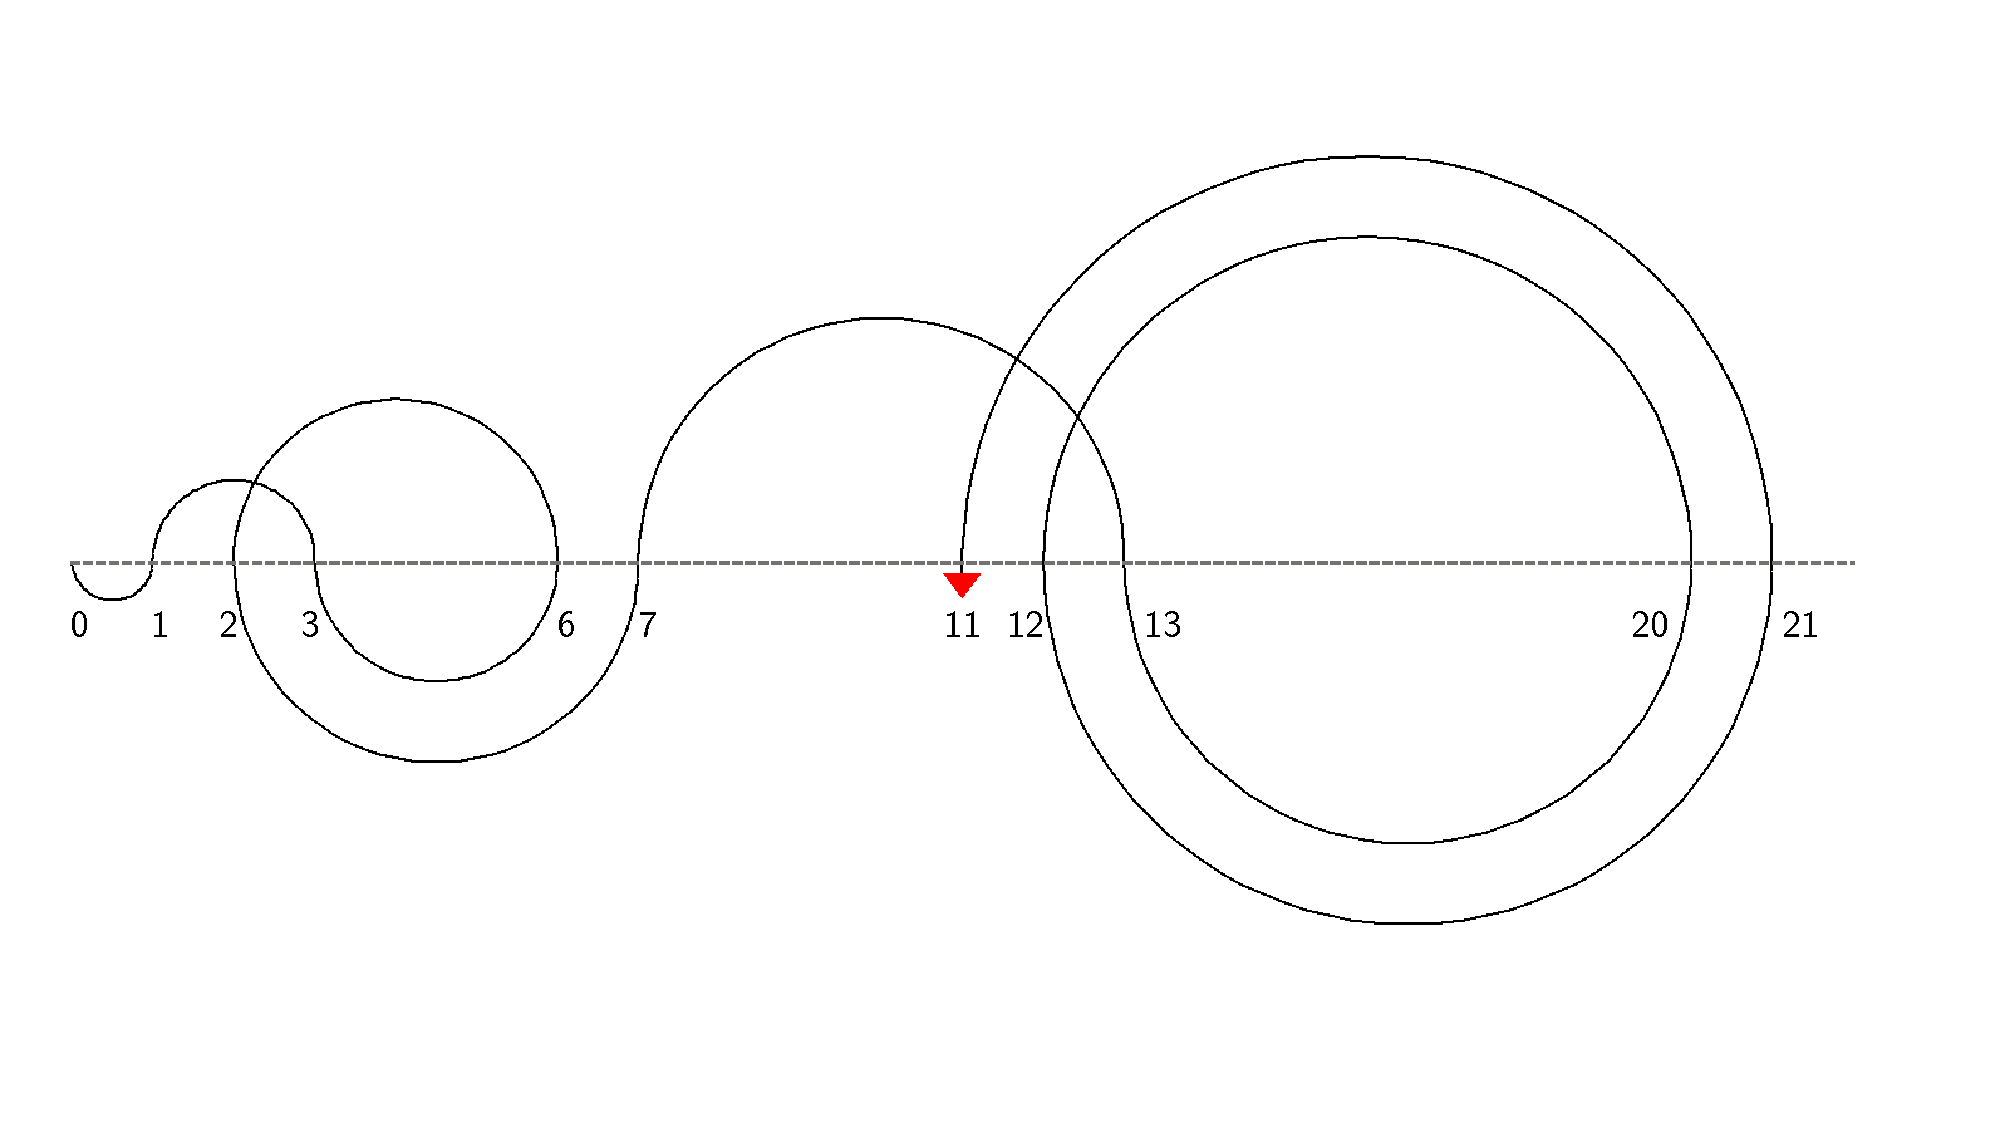
\includegraphics[width=0.7\linewidth]{Recaman's Sequence.pdf}
	\caption{Recaman's Sequence Drawing Procedure}
	\label{fig:recamanssequence}
\end{figure}
\begin{itemize}
\item Create a canvas named ``Recamans Sequence'' with width=1920, and height=1080.
\item Connect all consecutive terms using semicircles.
\item The semicircles should be parallel to $x-$axis with end points as consecutive terms
\item The semicircles should alternate above and below the $x-$axis; i.e., it should be below the axis when connecting $r_0, r_1,$ above the axis when connecting $r_1, r_2,$ again below for $r_2, r_3,$ and so on.
\item The figure should be dynamic; i.e., the $x-$axis should be such that for any $n$ the figure takes up at least half the canvas and it also remains within the canvas.
\item Don't draw the numbers and the axis. They are just to visualise the construction.
\end{itemize}
\textbf{Problem Statement:}\\
Generate the first $n+1$ elements $r_0,r_1,\ldots,r_n$ of the Recaman's Sequence and draw the corresponding curve using \verb!turtleSim!.
\begin{testcasesMore}
	{$n$ \hfill(a single integer)}
	{First $n+1$ elements of the Recaman's sequence and the curve.}
	{$1 \leq n \leq 1000$}
	{60}
	{0 1 3 6 2 7 13 20 12 21 11 22 10 23 9 24 8 25 43 62 42 63 41 18 42 17 43 16 44 15 45 14 46 79 113 78 114 77 39 78 38 79 37 80 36 81 35 82 34 83 33 84 32 85 31 86 30 87 29 88 28}
	{https://github.com/paramrathour/CS-101/tree/main/Test Cases/Recaman's Sequence/Input}
	{https://github.com/paramrathour/CS-101/tree/main/Test Cases/Recaman's Sequence/Output}
	{https://github.com/paramrathour/CS-101/tree/main/Starter Codes/Recaman's Sequence.cpp}
\end{testcasesMore}
\textbf{The output curve}
\begin{figure}[H]
	\centering
	\begin{subfigure}{0.3\linewidth}
		\includegraphics[width = \linewidth]{Recaman's Sequence/10.png}
		\caption{$n=10$}
	\end{subfigure}
	\begin{subfigure}{0.3\linewidth}
		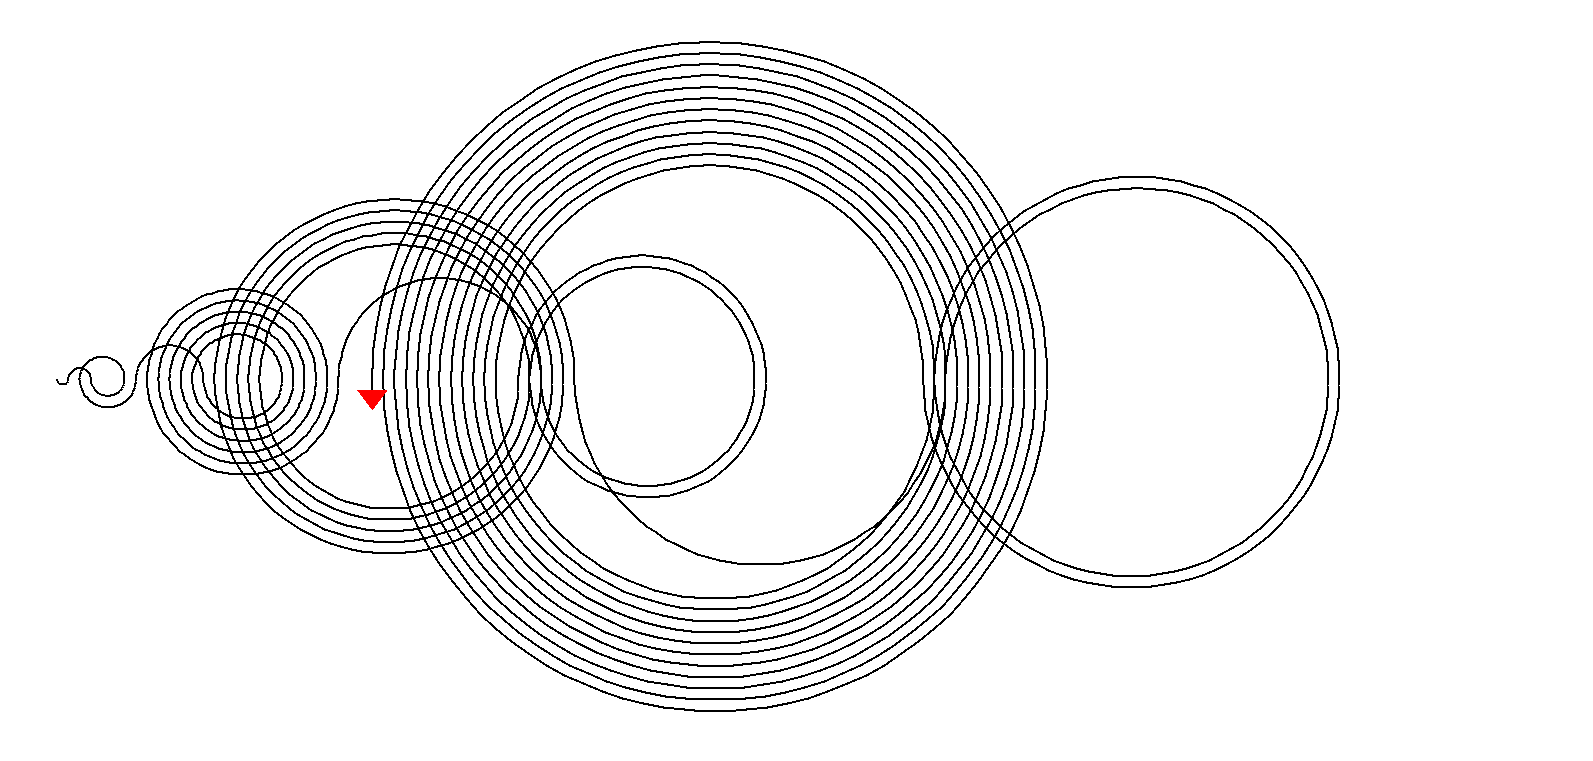
\includegraphics[width = \linewidth]{Recaman's Sequence/60.png}
		\caption{$n=60$}
	\end{subfigure}
	\begin{subfigure}{0.3\linewidth}
		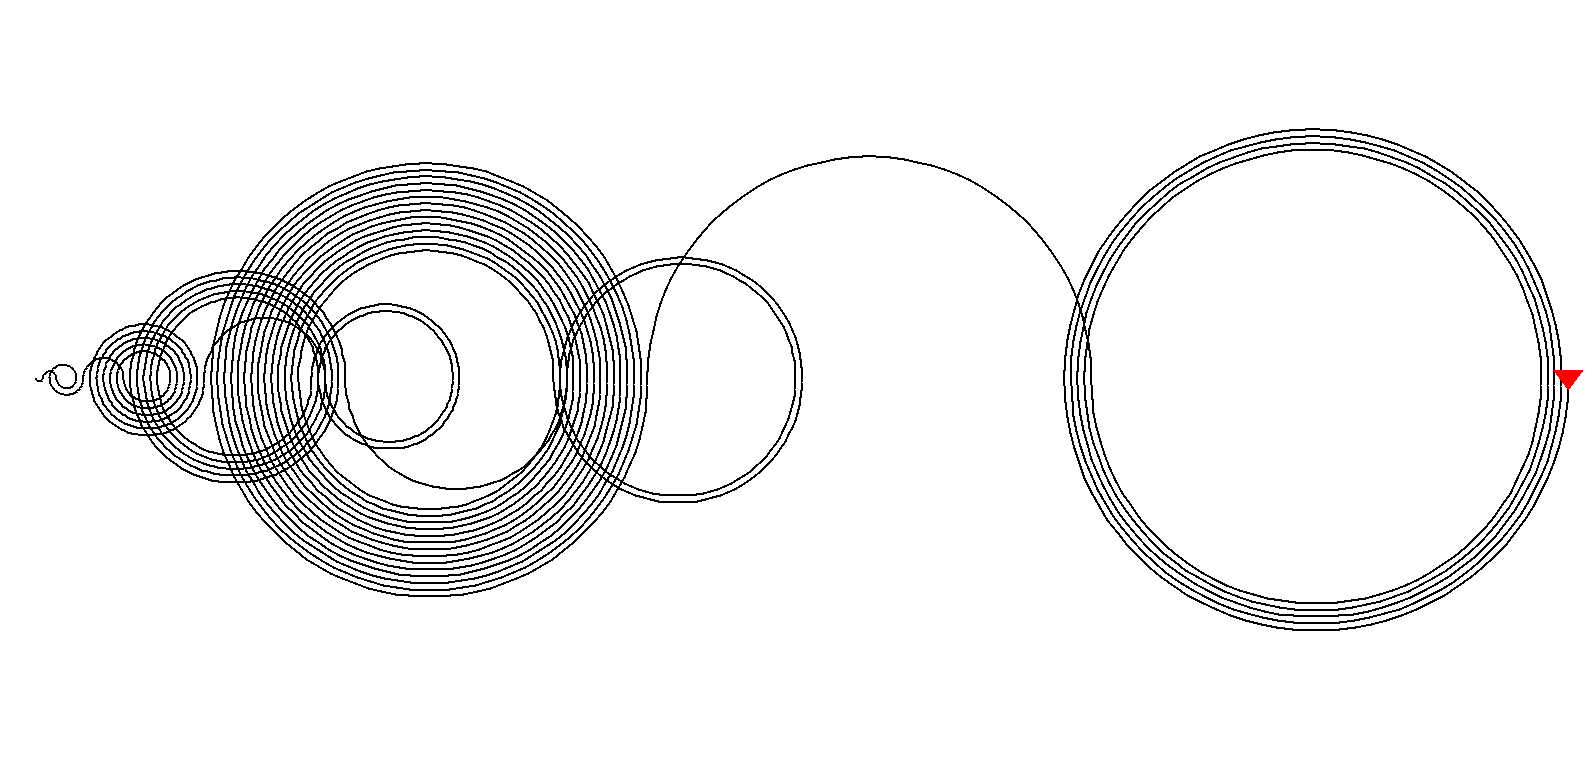
\includegraphics[width = \linewidth]{Recaman's Sequence/75.png}
		\caption{$n=75$}
	\end{subfigure}
	\caption{Output Ford Circles for few $n$}
\end{figure}
\begin{funvideo}
	\href{https://youtu.be/FGC5TdIiT9U}{The Slightly Spooky Recamán Sequence -- Numberphile}
\end{funvideo}
\subsection{Farey Sequence}{\label{pp:fareysequence}}
Farey sequence has all rational numbers in range $[0/1\ \text{to}\ 1/1]$ sorted \emph{in increasing order} such that the denominators are less than or equal to $n$ and all numbers are in \emph{reduced forms} i.e., 2/4 does not belong to this sequence as it can be reduced to 1/2.\\
For example, $n=4$, the possible rational numbers in increasing order are $\ 0/1,\ 1/4,\ 1/3,\ 1/2,\ 2/3,\ 3/4,\ 1/1$.
\vspace{-1em}
\subsubsection*{Stern-Brocot Tree}
\vspace{-0.7em}
To generate the Farey Sequence, we have to first look at the {Stern-Brocot Tree} shown in \ref{fig:sternbrocottree}.
\begin{figure}[H]
	\centering
	\scalebox{1}[0.8]{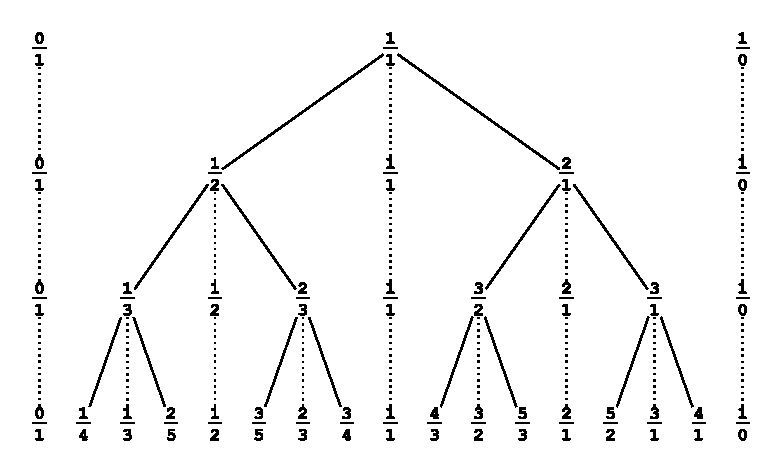
\includegraphics[width=0.6\linewidth]{Stern-Brocot Tree.pdf}}
	\caption{The Stern-Brocot Tree for Level $1-4$ (\href{https://commons.wikimedia.org/wiki/File:SternBrocotTree.svg}{Image} by \href{https://commons.wikimedia.org/wiki/User:Aaron_Rotenberg}{Aaron Rotenberg} licensed under \href{https://creativecommons.org/licenses/by-sa/3.0/}{CC BY-SA 3.0})}
	\label{fig:sternbrocottree}
\end{figure}
In this tree, a child is given by the \href{https://en.wikipedia.org/wiki/Mediant_(mathematics)}{mediant} of their parents; i.e, for child of parents $\mfrac{a}{c}$ and $\mfrac{b}{d}$ is $\mfrac{a+b}{c+d}$.

Some examples for parent, child are as follows -- $\left(\mfrac{0}{1}, \mfrac{1}{1} \rightarrow \mfrac{1}{2}\right)$, $\left(\mfrac{1}{1}, \mfrac{1}{0} \rightarrow \mfrac{2}{1}\right)$, $\left(\mfrac{0}{1}, \mfrac{1}{2} \rightarrow \mfrac{1}{3}\right)$, $\left(\mfrac{1}{2}, \mfrac{1}{1} \rightarrow \mfrac{2}{3}\right)$, $\left(\mfrac{1}{1}, \mfrac{2}{1} \rightarrow \mfrac{3}{2}\right)$, $\left(\mfrac{2}{1}, \mfrac{1}{0} \rightarrow \mfrac{3}{1}\right)$,

Notice that the farey sequence for corresponding $n$ is the subset of vertices of this tree calculated upto level $n$.

Also, for every fraction $\mfrac{p}{q}$ in the farey sequence draw a circle with centre at $\left(\mfrac{p}{q}, \mfrac{1}{2q^2}\right)$ and radius $\left(\mfrac{1}{2q^2}\right)$. You may need to do some scaling to get a proper figure.

\textbf{Problem Statement:}\\
Generate the Farey Sequence for corresponding $n$ using ideas from the Stern-Brocot Tree or otherwise and draw the circles.
\begin{hint}
	Recursion!
\end{hint}
\begin{testcasesMore}
	{$n$ \hfill(a single integer)}
	{Corresponding numbers in farey sequence in $p/q$ format with the circles.}
	{$1\leq n\leq 30$ \hfill(an integer)}
	{7}
	{0/1 1/7 1/6 1/5 1/4 2/7 1/3 2/5 3/7 1/2 4/7 3/5 2/3 5/7 3/4 4/5 5/6 6/7 1/1}
	% {0/1 1/1\\0/1 1/2 1/1\\0/1 1/3 1/2 2/3 1/1\\0/1 1/4 1/3 1/2 2/3 3/4 1/1\\0/1 1/5 1/4 1/3 2/5 1/2 3/5 2/3 3/4 4/5 1/1\\0/1 1/6 1/5 1/4 1/3 2/5 1/2 3/5 2/3 3/4 4/5 5/6 1/1\\0/1 1/7 1/6 1/5 1/4 2/7 1/3 2/5 3/7 1/2 4/7 3/5 2/3 5/7 3/4 4/5 5/6 6/7 1/1\\0/1 1/8 1/7 1/6 1/5 1/4 2/7 1/3 3/8 2/5 3/7 1/2 4/7 3/5 5/8 2/3 5/7 3/4 4/5 5/6 6/7 7/8 1/1\\0/1 1/13 1/12 1/11 1/10 1/9 1/8 1/7 2/13 1/6 2/11 1/5 2/9 3/13 1/4 3/11 2/7 3/10 4/13 1/3 4/11 3/8 5/13 2/5 5/12 3/7 4/9 5/11 6/13 1/2 7/13 6/11 5/9 4/7 7/12 3/5 8/13 5/8 7/11 2/3 9/13 7/10 5/7 8/11 3/4 10/13 7/9 4/5 9/11 5/6 11/13 6/7 7/8 8/9 9/10 10/11 11/12 12/13 1/1\\0/1 1/21 1/20 1/19 1/18 1/17 1/16 1/15 1/14 1/13 1/12 1/11 2/21 1/10 2/19 1/9 2/17 1/8 2/15 1/7 3/20 2/13 3/19 1/6 3/17 2/11 3/16 4/21 1/5 4/19 3/14 2/9 3/13 4/17 5/21 1/4 5/19 4/15 3/11 5/18 2/7 5/17 3/10 4/13 5/16 6/19 1/3 7/20 6/17 5/14 4/11 7/19 3/8 8/21 5/13 7/18 2/5 7/17 5/12 8/19 3/7 7/16 4/9 9/20 5/11 6/13 7/15 8/17 9/19 10/21 1/2 11/21 10/19 9/17 8/15 7/13 6/11 11/20 5/9 9/16 4/7 11/19 7/12 10/17 3/5 11/18 8/13 13/21 5/8 12/19 7/11 9/14 11/17 13/20 2/3 13/19 11/16 9/13 7/10 12/17 5/7 13/18 8/11 11/15 14/19 3/4 16/21 13/17 10/13 7/9 11/14 15/19 4/5 17/21 13/16 9/11 14/17 5/6 16/19 11/13 17/20 6/7 13/15 7/8 15/17 8/9 17/19 9/10 19/21 10/11 11/12 12/13 13/14 14/15 15/16 16/17 17/18 18/19 19/20 20/21 1/1}
	{https://github.com/paramrathour/CS-101/tree/main/Test Cases/Farey Sequence/Input}
	{https://github.com/paramrathour/CS-101/tree/main/Test Cases/Farey Sequence/Output}
	{https://github.com/paramrathour/CS-101/tree/main/Starter Codes/Farey Sequence.cpp}
\end{testcasesMore}
\textbf{The output circles (Ford Circles)}
\begin{figure}[H]
	\centering
	\begin{subfigure}{0.3\linewidth}
		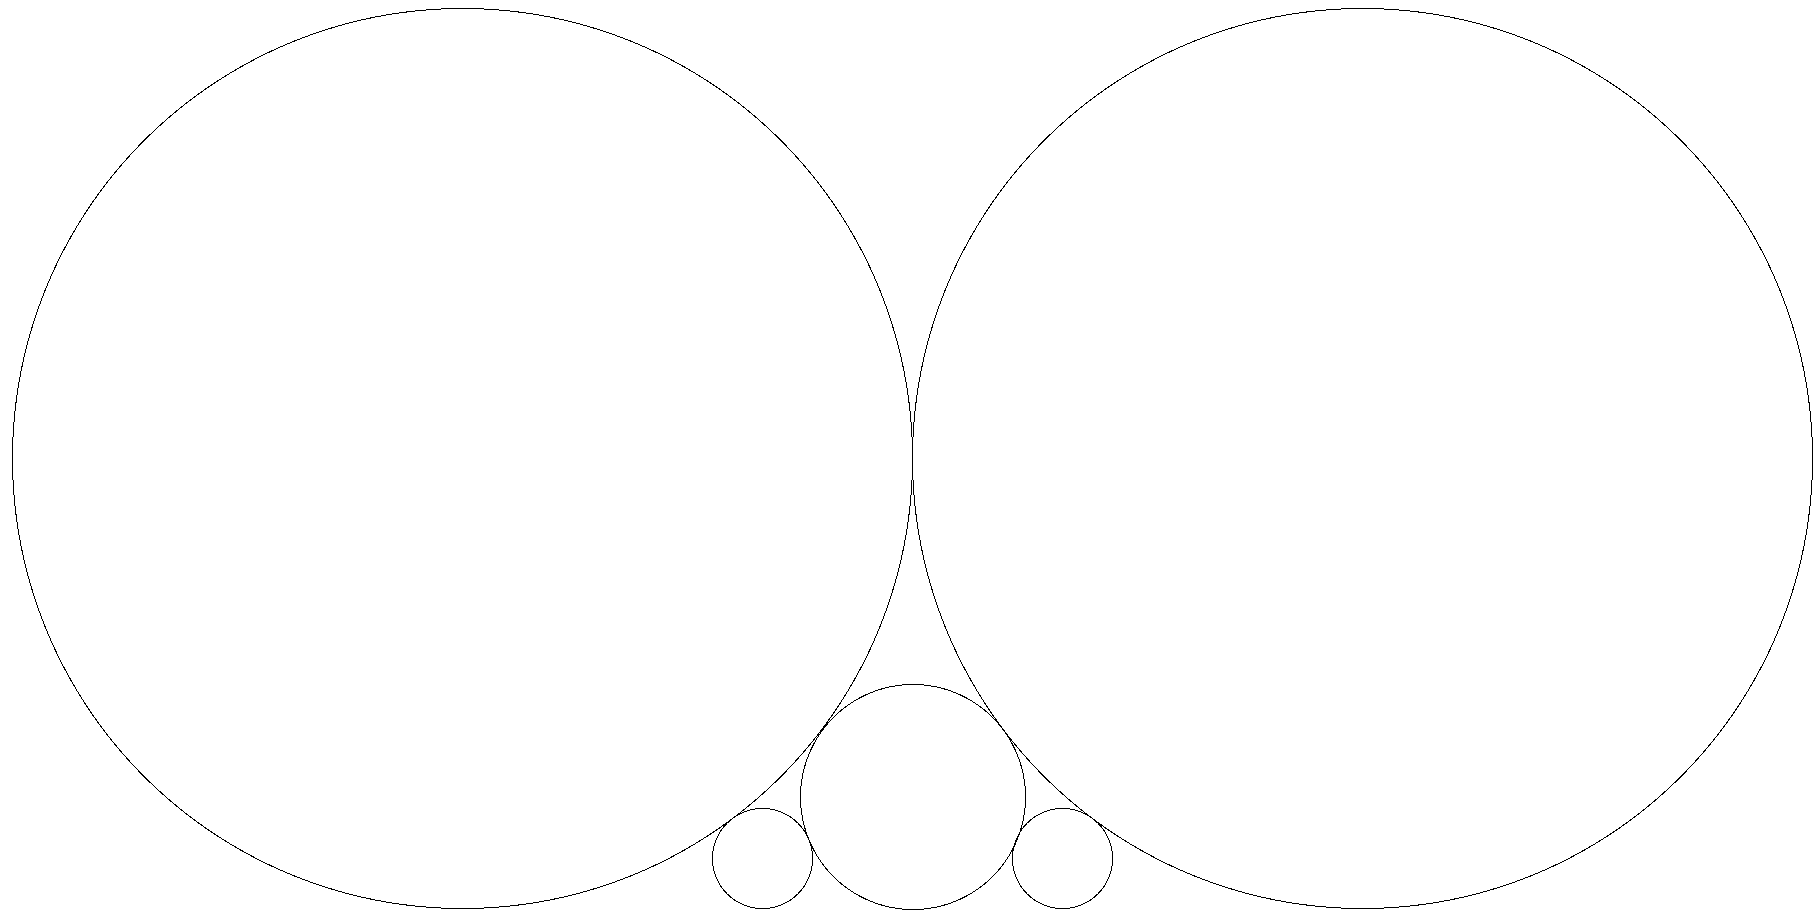
\includegraphics[width = \linewidth]{Farey Sequence/3.png}
		\caption{$n=3$}
	\end{subfigure}
	\begin{subfigure}{0.3\linewidth}
		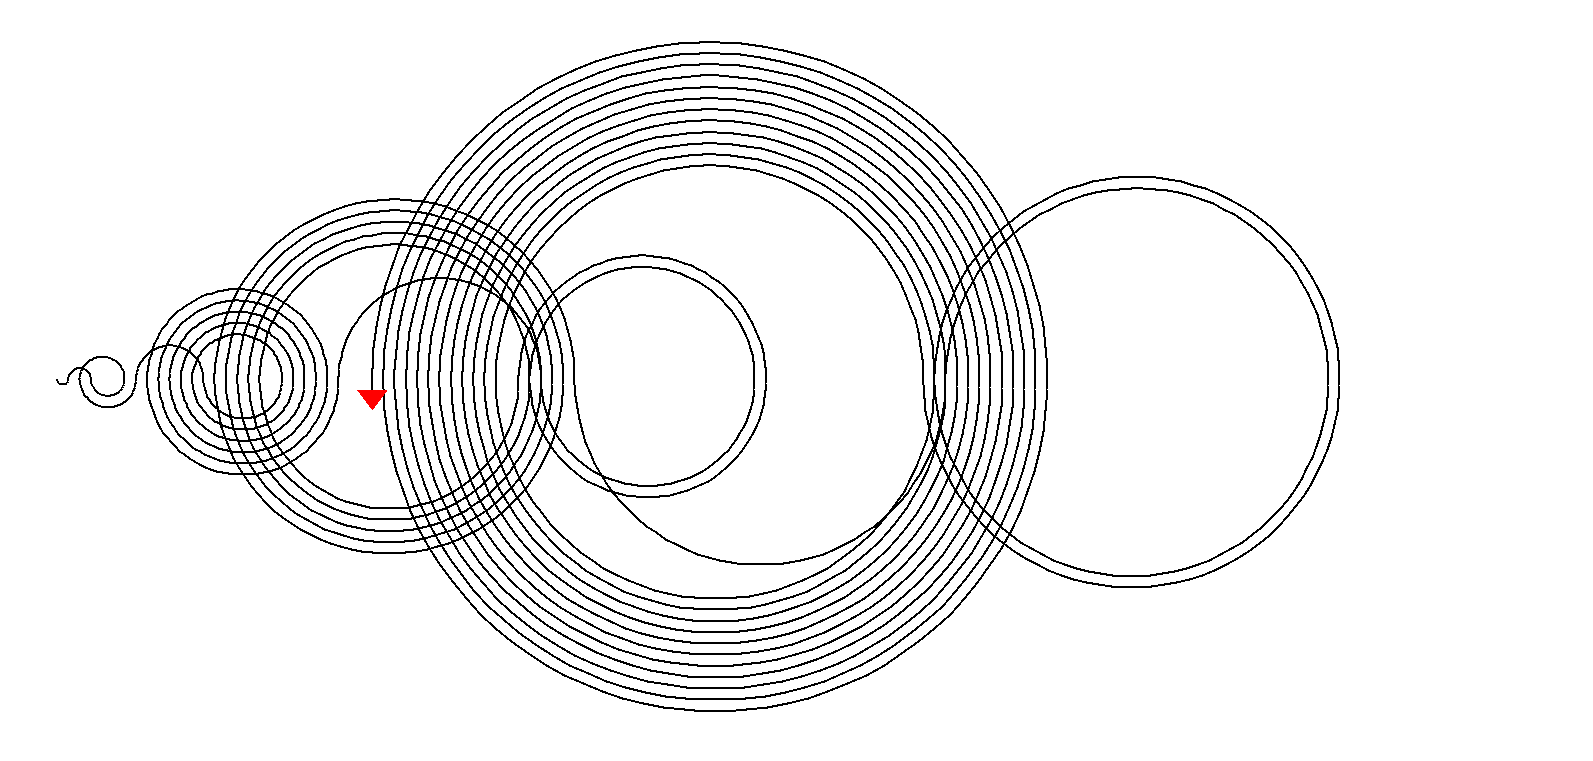
\includegraphics[width = \linewidth]{Farey Sequence/7.png}
		\caption{$n=7$}
	\end{subfigure}
	\begin{subfigure}{0.3\linewidth}
		\includegraphics[width = \linewidth]{Farey Sequence/10.png}
		\caption{$n=10$}
	\end{subfigure}
	\caption{Output Ford Circles for few $n$}
\end{figure}
\begin{noteI}
	If the outputs take a long time then how can you make it faster?. Also, try calculating terms mathematically to get the fastest way!
\end{noteI}
\begin{funvideo}
\href{https://youtu.be/DpwUVExX27E}{Infinite Fractions -- Numberphile}\\
\href{https://youtu.be/0hlvhQZIOQw}{Funny Fractions and Ford Circles -- Numberphile}
\end{funvideo}
\KOMAoptions{paper=A4}
\recalctypearea